
% This is a sample document using the University of Minnesota, Morris, Computer Science
% Senior Seminar modification of the ACM sig-alternate style. Much of this content is taken
% directly from the ACM sample document illustrating the use of the sig-alternate class. Certain
% parts that we never use have been removed to simplify the example, and a few additional
% components have been added.

% See https://github.com/UMM-CSci/Senior_seminar_templates for more info and to make
% suggestions and corrections.

\documentclass{sig-alternate}
\usepackage{color}
\usepackage[colorinlistoftodos]{todonotes}
\usepackage[linesnumbered]{algorithm2e}
\usepackage{listings}

\definecolor{dkgreen}{rgb}{0,0.6,0}
\definecolor{gray}{rgb}{0.5,0.5,0.5}
\definecolor{mauve}{rgb}{0.58,0,0.82}

\lstset{frame=tb,
  language=Java,
  aboveskip=3mm,
  belowskip=3mm,
  showstringspaces=false,
  columns=flexible,
  basicstyle={\tiny\ttfamily},
  numbers=none,
  numberstyle=\tiny\color{gray},
  keywordstyle=\color{blue},
  commentstyle=\color{dkgreen},
  stringstyle=\color{mauve},
  breaklines=true,
  breakatwhitespace=true,
  tabsize=3
}

\let\oldnl\nl% Store \nl in \oldnl
\newcommand{\nonl}{\renewcommand{\nl}{\let\nl\oldnl}}% Remove line number for one line

%%%%% Uncomment the following line and comment out the previous one
%%%%% to remove all comments
%%%%% NOTE: comments still occupy a line even if invisible;
%%%%% Don't write them as a separate paragraph
%\newcommand{\mycomment}[1]{}

\begin{document}

% --- Author Metadata here ---
%%% REMEMBER TO CHANGE THE SEMESTER AND YEAR AS NEEDED
\conferenceinfo{UMM CSci Senior Seminar Conference, December 2017}{Morris, MN}

\title{Thread Scheduler Efficiency Improvements \\ for Multicore Systems}

\numberofauthors{1}

\author{
% The command \alignauthor (no curly braces needed) should
% precede each author name, affiliation/snail-mail address and
% e-mail address. Additionally, tag each line of
% affiliation/address with \affaddr, and tag the
% e-mail address with \email.
\alignauthor
Daniel C. Frazier\\
	\affaddr{Division of Science and Mathematics}\\
	\affaddr{University of Minnesota, Morris}\\
	\affaddr{Morris, Minnesota, USA 56267}\\
	\email{frazi177@morris.umn.edu}
}
\maketitle

\begin{abstract}

Thread scheduling is a problem that has been around since the 1960s. By the early 2000s, thread scheduling was commonly believed to be solved in the Linux community. However, with the rising popularity of multiprocessor and multicore systems, and the rapidly developing requirements driven by new hardware, the problem space has become considerably more complex. This paper will describe some newly found issues in the Linux scheduler, their fixes, and two new schedulers designed for improved performance. Each of the developments meaningfully improve the average efficiency of popular relevant benchmarks.

\end{abstract}

\keywords{Scheduling; thread migration; multicore; multiprocessing; lock contention; last-level cache misses; efficiency}

\section{Introduction}
\label{sec:intro}

Using any modern computer, there is an expectation that the operating system is running at all times (largely in the background) and that multiple programs should be able to run concurrently. Modern programs also often need to run more than one independent task at one time. A program can achieve this by employing \emph{threads}. Programs that involve long independent computations or programs with a graphical interface often benefit from employing threads.

For example, imagine a photo editing program that can apply an expensive filter operation. If the program wasn't multithreaded, the user interface and the filter operation would be executed in the same thread. When instructing the program to execute the filter on a large image, the user interface wouldn't be able to respond to any events (like clicking the mouse) until filtering was finished. To make GUI programs more responsive, we separate the UI onto its own thread and spawn new threads when the user initiates expensive operations.

There are many choices of hardware for a given computational problem. Processors on most modern computing systems employ multiple cores. Some systems have multiple processors, each of which also have multiple cores. To take advantage of this hardware, threads should be distributed across the cores wisely.

In \emph{The Linux Scheduler: a Decade of Wasted Cores}, Lozi et al. describe bugs they found within the Linux scheduler that resulted in significant performance degradation over time. In this paper, we will cover some important decisions and trade-offs that are made in order to allocate tasks to cores to maximize performance. In the next section, we will provide necessary background on threads, scheduling, and caching. In section \ref{sec:methods} we will discuss the bugs (and their fixes) and approaches by Kumar et al. and Jo et al. to create new schedulers that overcome scalability problems with the Linux scheduler.
\section{Background}
\label{sec:bg}

In this section, we will broadly establish how threading, caching, and scheduling works. These concepts will prepare us to establish causes of something called cache misses in the execution of programs using the current Linux thread scheduler. We will establish information necessary to understand some recent efforts made to improve thread scheduling on multiprocessor and multicore systems on Linux.

\subsection{Threads and Scheduling}
\label{sec:threads}

Threads are tied to the \emph{processes} that spawn them. A process always has at least one thread. Processes are typically independent of each other while threads exist within a process. \emph{Context switching} within a CPU is the process of storing and restoring the state of a process or thread so that execution can be paused or resumed. A process's state consists of resources that each of its threads should have access to, dominantly compiled code and data. A thread's state is used at runtime but is also stored to pause or resume a thread's execution.

The \emph{scheduler} is the part of the operating system that is responsible for managing and distributing the CPU runtime which each of these processes and their respective threads receive. New threads and processes are added to the scheduler when they are made.~\cite{Lozi:2016} The current implementation of the scheduler on Linux is hierarchical and consists of modules. The primary module is the \emph{scheduler core}, and it interfaces with modules called \emph{scheduler classes}. The \emph{Completely Fair Scheduler (CFS)} is the default scheduler class and is used for tasks that are not real-time critical. The core scheduler runs a tick function that runs $\sim1000$ times per second and calls the tick function of the appropriate scheduler class. For real-time tasks, the First-in first-out (FIFO) or Round-Robin (RR) scheduler classes are used but out of brevity we will not be covering these.~\cite{SchedThesis}

Before we discuss how the CFS schedules tasks, we should first understand how and where cache exists on most multicore systems, how a system can maintain cache coherence, how threads can work on the same data without conflicting with each other, and a few other related system performance concepts.

\subsection{Cache on NUMA Systems}
\label{sec:cache}

When a program is running, its memory is stored in RAM. RAM exists far away from the CPU relative to the~\emph{cache}. Imagine a program that sums up an array of ten thousand integers and they all fit into RAM. It would be very slow for the CPU to request from RAM integers one at a time. Cache exists to speed this up by improving \emph{locality}. If the system predicts a chunk of data will be used frequently, it migrates that data from the RAM into cache. This improves locality because it makes the data more ``local'' to where it needs to be and improves performance because the system works less hard to load the data it needs.

The cache that a system has is hardware dependent. Cache can be integrated into, on top of, or outside of a core or processor. In a \emph{non-uniform memory access (NUMA)} system, there are many levels of cache and they exist in a hierarchy. The defining property of NUMA systems is that levels of cache that are physically closer to cores or processors are faster than levels that are farther. Lower levels of cache also hold less data because of space restrictions. Most modern systems are multiprocessor multicore NUMA systems. Levels of cache are labeled [L1, L2,\dots, Ln] where L1 is nearest to the CPU. See Figure \ref{fig:cache} for an example of a NUMA setup.

\begin{figure}
\centering
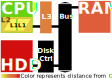
\psfig{file=CacheAbstract.pdf,width =3in}
\caption{Example cache setup for a dual-core processor system with three levels of cache}
\label{fig:cache}
\end{figure}

L1 cache is also called last \emph{level cache (LLC)}. If data is not found in L1 cache, it is called an \emph{LLC miss} and the data is searched for in L2 cache and so on. If the data can not be found in any level of cache, it is called a \emph{cache miss} and external memory is consulted for the data. 

An important property of a multicore system that employs cache is that it should be \emph{cache coherent}. A system that is cache coherent satisfies the invariant that any data that is \emph{read} that pertains to a certain portion of cached data must be consistent with the most recent \emph{write} to that portion of data. When data is written into an L1 cache, it must propagate to its parent caches. If any \emph{other} L1 cache holds the same data as that L1 cache, it must also refresh. The most common approach to maintain strict consistency in cache is to somehow \emph{invalidate} cache entries. How cache invalidation works is out of the scope of this paper~\footnote{See Section 10.2.4 in Part II of Principles of Computer System Design by Saltzer, Jerome and Kaashoek, M. Frans for more information on cache invalidation.}.~\cite{Systems}

Context switching between two cores involves ensuring that the replacing thread has the resources it needs available on its new core's cache. Recall that a processor's state is much larger than thread's state. Because of this, context switching is typically fastest between threads who share a process because the processor's state wouldn't need to migrate to another cache.

A NUMA system has \emph{NUMA nodes}, but the definition of what a NUMA node is changes depending on how NUMA is implemented on a machine. So let us consider how NUMA nodes were defined for the system used in Lozi et al. On their system, groups of eight cores share last level cache and form a NUMA node.

\subsection{Synchronicity and Locks}
\label{sec:locks}

When two threads have \emph{read} and \emph{write} access to the same portion of the memory, any \emph{read} or \emph{write} to that memory must be made synchronous to avoid race conditions. A race condition is a timing dependent error where two threads updating the same memory at the same time overwrite each other in a way that might cause the threads to function incorrectly. A system can be made synchronous by employing \emph{locks}. \textit{Principles of Computer System Design} by Saltzer and Kaashoek defines locks as ``A flag associated with a data object, set by a thread to warn concurrent threads that the object is in use and that it may be a mistake for other threads to read or write it.''~\cite{Systems}
When a thread needs to use an object which is associated with a lock, the thread should check the lock first before operating on the object. If an object's lock is already acquired, the thread should wait until the lock is released, then acquire it for itself.

An important problem faced by massively parallel programs is called lock contention. \emph{Lock contention} can be found in multithreaded programs where many threads frequently compete for access to the same lock. Threads of a program that are contending and which reside on different processors experience a higher than average LLC miss rate. This is a result of cache coherency. Because both of these threads are continually modifying the same data in separate cache, each change to one cache must propagate to the other before the other core reads the data.


\subsection{Completely Fair Scheduler (CFS)}
\label{sec:cfs}

The \emph{Completely Fair Scheduler (CFS)} was introduced in version 2.6.23 of the Linux kernel.~\cite{Jo:2017} We will discuss the CFS as presented in Lozi et al. The CFS is an implementation of the weighted fair queuing (WFQ) scheduling algorithm. The goal of the WFQ is to divide an arbitrary number of CPU cycles among threads, prioritizing more cycles for threads with larger weights.~\cite{Lozi:2016}

Threads that are running accumulate \emph{vruntime}, which is the runtime of a thread divided by its weight.~\cite{SchedThesis} Threads are organized in priority queues called \emph{runqueues} that sort ascending on vruntime. Under normal conditions, the thread that replaces the current thread is the thread which needs most to run, which is the thread with the least vruntime, the first thread in the runqueue. If a thread with a smaller vruntime awakens, it may preempt the executing thread.~\cite{Lozi:2016}

On a multicore system, each core should have its own runqueue. If all cores shared a runqueue, cores would be need to make frequent synchronous requests for threads. For the scheduler to function properly and efficiently, it must keep each of the runqueues balanced. If runqueues are not balanced, then a core is left idle and needs to request work from another core to keep busy. External calls between cores are expensive and should be minimized. The CFS, runs a load-balancing algorithm that tries to keep runqueues balanced. Load balancing was simple for single-core systems, but on multi-core systems, bugs have found their way into the system and persist until at least Linux kernel version 4.3.~\cite{Lozi:2016}

\begin{quote}
Our recent experience with the Linux scheduler revealed that the pressure to work around the challenging properties of modern hardware, such as non-uniform memory access latencies (NUMA), high costs of cache coherency and synchronization, ... resulted in a scheduler with an incredibly complex implementation. As a result, the very basic function of the scheduler, which is to make sure that runnable threads use idle cores, fell through the cracks.~\cite{Lozi:2016}
\end{quote}

\section{Methods}
\label{sec:methods}

So far we have established what threads are, how cache works and where it resides on NUMA systems, how the CFS scheduler works, how locks work and why they are important. Now, we will discuss four bugs Lozi et al. found in the CFS load-balancer and their fixes, which substantially improved scheduler efficiency. Later, we will show two new schedulers that improve efficiency for certain kinds of programs running on certain kinds of multicore NUMA systems.

\subsection{Load-Balancing the CFS}
\label{sec:loadbalance}

Modifications were made to the CFS load balancer that introduced bugs that caused processors to remain idle even when there were threads available. Work by Lozi et al. has identified four bugs that were responsible for this behavior. These bugs have remained hidden because, while they corrode performance, they are not obvious. They do not make programs freeze or crash and their effects only last a few hundred milliseconds at a time, which is too short for common performance tools to detect. Lozi et al. designed new tools that observe the Linux scheduler more closely. These tools helped them isolate the problems.~\cite{Lozi:2016}

In order to understand these bug fixes, as described in Lozi et al., we must explain a simplified version of the CFS load balancer.~\cite{Lozi:2016}

\subsubsection{Load Metric}
\label{sec:loadmetric}

The load-balancing algorithm tracks a metric called \emph{load} to best distribute threads to cores. Defining what load should be is tricky. A threads' load should be representative of the amount of CPU time it should receive relative to all other active threads. Balancing load such that each core has the same number of threads is not ideal because threads have priorities, and if all of the high-priority threads happened to be placed on one core while all low-priority threads were placed on another, the low-priority threads would be receiving much more runtime than they should be in relation to the high-priority threads. Balancing load such that each core has roughly the same amount of weight is not ideal either, because, if there was one thread that was nine times more important than nine low-priority threads, that important thread would be left on a core all alone. That seems acceptable, but consider the case that this high-priority thread sleeps frequently. Its core would be left idle for an unacceptable amount of time. The idle core would need to ask other cores for more work to keep busy in the downtime, which is an expensive operation for both cores involved.~\cite{Lozi:2016}

The current implementation of CFS defines the load metric as a combination of a thread's weights and average CPU use divided by the number of all threads in the parent process. The division is in order to remain fairness so that two processes which have different numbers of threads of the same priority still get equal runtime.~\cite{Lozi:2016}

\subsubsection{Load-Balancing Algorithm}
\label{sec:loadbalancealg}

\begin{figure}
\centering
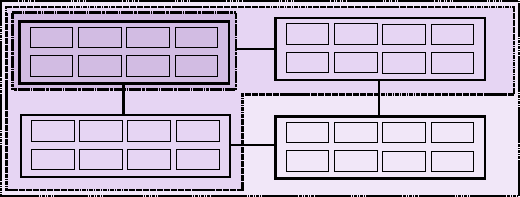
\psfig{file=NUMA.pdf,width =3in}
\caption{32-core machine with four NUMA nodes. It only takes two hops to get from any core to another node. The shades represent scheduling domains relative to the first core. From Lozi et al.~\cite{Lozi:2016}}
\label{fig:domains}
\end{figure}

For load balancing, cores exist in a hierarchy where each level is called a \emph{scheduling domain}. The groups within each level are based on how cores share resources within the machine. The lowest level of scheduling domain is a single core. A \emph{scheduling group} is one of the units that comprise a scheduling domain. In the machine described in Section~\ref{sec:cache} there were 32 cores. These cores individually represented the first level of scheduling domains. The second scheduling domains were determined by groups of eight adjacent processors which made four NUMA nodes. The third level was formed by groupings of nodes that are within one hop of each other. The final level was all of the nodes as one unit. The scheduling groups of the final scheduling domain were the four NUMA nodes. See Figure~\ref{fig:domains}.~\cite{Lozi:2016}


{\SetAlgoNoLine%
	\DontPrintSemicolon 
\begin{algorithm}
\nonl Function running on each cpu $\textit{cur\_cpu:}$\;
	\ForAll{sd in sched\_domains of cur\_cpu}{
		\eIf{sd has idle cores}{first\_cpu = $1^{st}$ idle CPU of sd}
		{
			first\_cpu = $1^{st}$ CPU of sd\;
		}
		\If{cur\_cpu $\neq$ first\_cpu}{
			$\textbf{continue}$\;
		}
		\ForAll{sched\_group sg $\textbf{in}$ sd}{
			sg.load = average loads of CPUs in sg\;
		}
		busiest = overloaded sg with the highest load\;
			\nonl\quad($\textbf{or}$, if inexistent) imbalanced sg with highest load\;
			\nonl\quad($\textbf{or}$, if inexistent) sg with the highest load\;
		local = sg containing cur\_cpu\;
		\If{busiest.load $\leq$ local.load}{
			$\textbf{continue}$
		}
		busiest\_cpu = pick busiest cpu of sg\;
		try to balance load between busiest\_cpu and cur\_cpu\;
		\If{load cannot be balanced due to tasksets}{
		exclude busiest\_cpu, $\textbf{goto}$ line 18
		}
	}
\label{fig:cfsloadbalancer}	
\caption{Simplified CFS Load Balance algorithm from Lozi et al.~\cite{Lozi:2016} CPUs are cores.}
\end{algorithm}
}

A naive approach to load balancing would be to compare load on each core and transfer tasks from cores with the highest load to cores with the lowest load. This approach would not put into consideration improving thread or cache locality. Instead, the CFS load-balancing algorithm is executed on each CPU for each scheduling domain that the CPU is a part of, starting from the first level to last levels of scheduling domain. A simplification of the CFS load balancing algorithm can be found in Algorithm \ref{fig:cfsloadbalancer}. The goal of each iteration of the outer loop is to find another CPU that is busier than \emph{cur\_cpu} and ``try to balance load'' between them. This simplification does not cover the intricacies of load balancing, however is sufficient for understanding the bugs that emerged.

In the CFS load balancer, one core per scheduling domain performs the load-balancing for that domain. That core is either the first core that is idle or the first core of the scheduling domain (Lines 2-9). Then for each scheduling group within the scheduling domain, the average load is computed (Lines 10-12) and the group with the highest load is determined to be the busiest group (Line 13). If the busiest group is less busy than the group containing this CPU (local), then the load is considered balanced for this level and continues on to consider the next scheduling domain (Lines 14-17). At lines 18 to 23 the current core balances load between the bustiest core and itself.~\cite{Lozi:2016}

Several optimizations made the scheduler such that it runs the load balancing operation less often. Lines 2-8 is an example of this where if any of the cores are idle, the first idle core in the scheduling domain is chosen to consider load balancing. If all cores are busy, the first core of the scheduling domain is chosen. There is also a power optimization where idle cores don't run the load balancing algorithm until awoken by an overloaded core. To improve cache locality, when an idle thread is awoken by an active thread, the scheduler prefers to assign the awoken thread to the same core so that they share a last-level cache.~\cite{Lozi:2016}

\subsection{Bugs and Fixes for the CFS}
\label{sec:cfsbugs}

Now that we know how the load balancer makes some decisions, we will now dive into the bugs that occur as a result of the complex, strict requirements that have built up over time on the CFS. Performance results from Lozi et al. were gathered using the \emph{NAS Parallel Benchmark (NPB)}. The NPB is a set of parallel programs that are executed and monitored to evaluate the efficiency of massively parallel computing systems (supercomputers).

\subsubsection{The Group Imbalance bug}
\label{sec:cfsfault_grpimbalance}

Lozi et al. found that the scheduler was periodically not balancing load due to two reasons. The hierarchical design and complexity of the load metric. The researchers were running a 64 threaded Process A on node A simultaneously with a single-threaded Process B on node B. Because of group schedule feature in the definition of load metric where the load of a thread is divided by the number of threads in the parent process, the amount of load for each of A's threads are 1/64 of the load of the one B thread. On their system they observed that two nodes were underloaded and should have been stealing work from more loaded cores on other nodes, but this did not happen. This is due to the hierarchical design of the load balancer. When the load balancer considers stealing threads, it does not consider the load of a single core but rather the load of the whole scheduling group. In this case, the node with the B process had the same load as the node with the A process, so node B did not try to steal work from node A even though there were cores idle and available for work.~\cite{Lozi:2016}

They fixed this problem by instead of defining load of a scheduling group as the average load of cores in the group, it is defined by the load of the core with the minimum load in the scheduling group. By fixing this issue, the efficiency of the single-threaded process B remained the same, however the completion time of process A decreased by 13 percent. On a certain parallel program within the NPB called \textit{lu}, this bug fix improved performance by 13 times because the bug compounded lock contention by colocated threads.~\cite{Lozi:2016}

\subsubsection{The Scheduling Group Construction bug}
\label{sec:cfsfault_grpconstruct}

There is a function in Linux called taskset which allows an application to pin its threads to certain available cores. On certain machines, sequentially numbered NUMA nodes may be located more than one hop from each other. When a new thread is spawned on Linux, it is placed on the same node as the parent thread. The first scheduling group is constructed by all adjacent nodes to one node (say, Node 0), and following scheduling groups are constructed by adjacent nodes to nodes that were not in any of the previous groups. On a system it is possible for two nodes to be within one hop of the starting nodes of each group, but be two hops from each other. See Figure \ref{fig:cfs_schedgroups}.~\cite{Lozi:2016}

Within that system, the two scheduling groups constructed are {0,1,2,4,6} and {1,2,3,4,5,7}. Nodes 1 and 2 are two hops from each other but occur in both scheduling groups. When load balancing runs on Node 2 and it should steal work from an overloaded Node 1, it will look between the scheduling groups to compare which is lower. But both scheduling groups contain Node 1 and 2, so both scheduling groups' average load will be the same! Node 2 will never steal work.~\cite{Lozi:2016}

They fixed this bug by constructing scheduling groups relative to each core's own perspective. This allows nodes that are two hops away that should otherwise be able to share work to be a part of different scheduling groups and successfully contend for load balancing. Fixing this bug improved efficiency of 9 parallel programs in the NPB problems mostly by around 2 times, but for one problem, \textit{lu}, up to 27 times. \textit{lu} is an extreme example where all threads were being allocated only on one core.~\cite{Lozi:2016}

\begin{figure}
\centering
\psfig{file=CFS_AdjacentNodes.png,width =3in}
\caption{8-node AMD Bulldozer machine from Lozi et al.~\cite{Lozi:2016}}
\label{fig:cfs_schedgroups}
\end{figure}

\subsubsection{The Overload-on-Wakeup bug}
\label{sec:cfsfault_overload}


There exists an optimization in thread wake-up code where threads that are awakened by other threads are placed on the same core for improved cache locality. This becomes a problem when the core with the requesting thread is already overloaded. The thread will join the runqueue on this busy core rather than consider being migrated to an idle core elsewhere. For some workloads this is acceptable, but simply making the most of cache isn't always the best decision. This bug occurs primarily on database systems. The following sequence of events will illustrate how the Overload-on-Wakeup bug occurs.~\cite{Lozi:2016}

Consider two nodes running on a database system. Node A and Node B both have a database thread. Assume a temporary thread is created by the kernel on Node A for some background function such as system logging. During this time, the load balancer detects that the node is overloaded due to the new thread, and decides to migrate some thread to Node B. If it decides to move the temporary thread, that will pose no issue for performance. If it migrates the database thread, two database threads which sleep and awaken frequently will be running on the same node. The scheduler does not differentiate between cores that are idle for a short time versus a long time, so when the scheduler considers thread migration destinations, it might see a node, which happens to have a database thread that is currently idle, and decide that the node needs more work.~\cite{Lozi:2016}

Lozi et al. fixed this bug by modifying the thread wake up code. The scheduler first checks to see if the core that the thread was already assigned to is idle. If it is, then wake up the thread on that core. If the power manager policy of the system is set up so that cores never enter low-power mode and there are idle cores, the scheduler chooses the core that has been idle for the most time and assigns the thread to that core. This fix is only relevant to workloads where threads frequently sleep. Their fix improves performance by 13.2\% on a full TPC-H database workload but up to 22.2\% for certain queries.~\cite{Lozi:2016}

\subsubsection{The Missing Scheduling Domains bug}
\label{sec:cfsfault_missingsched}

This bug is actually something that was already fixed but regressed on Linux kernel version 3.19 (up to at least 4.3) when an important line of code was removed in a refactor that causes the system to misrepresent the number of scheduling domains that are available for assigning threads to. This ended up causing load-balancing to never happen on all nodes, meaning processes, subprocesses and their threads to stop looking for other NUMA nodes to assign themselves to. Nodes that do not have any threads will never receive threads and nodes that do have threads will accumulate all of the spawned threads.

This bug required that one of the cores become disabled and re-enabled. So while rare, reintroducing the removed line of code increased efficiency in a certain tested program by a maximum of 138 times.~\cite{Lozi:2016}

\subsection{Shuffler}
\label{sec:shuffler}

Researchers Kumar et al. suspected lock contention to be a significant actor in the non-scalability of parallel programs on Linux and Solaris. The operating system used was Oracle Solaris 11\textsuperscript{TM}. They assembled 33 parallel programs from various benchmarks and monitored time spent acquiring locks and the number of LLC misses experienced while running these programs. 20 of the 33 had high lock times~(>5\%).

As mentioned in the concepts section, lock contention can be found in multithreaded programs where many threads repeatedly compete for access to the same lock. The costs in this involve the transfer of the lock and the propagation of cache associated with the lock. The problem is further compounded if the threads are not located within the same processor. If the threads of that multithreaded program were prioritized to be placed on one processor, then the program would experience a lower lock times and LLC miss rate.

Neither the CFS nor the Solaris scheduler differentiate between threads of a single-threaded program versus the threads of a multithreaded program. This prevents the scheduler from using that metadata in its thread distribution mechanism. The following thread scheduler named \emph{Shuffler} by Kumar et al. takes this into account. The Shuffling framework was designed for multiprocessor multicore NUMA systems, and was implemented on a 64-core 4-processor machine running Oracle Solaris 11\textsuperscript{TM}.~\cite{Kumar:2014}

\subsection{The Shuffling Framework}

The Shuffling approach is to take into account which threads are contending for locks on what processors and migrate \textit{whole threads} (rather than lock and cache) such that they share processors. Threads that are reported to have higher lock acquisition times are threads that are assumed to be requesting locks from outside of their processor. These are the threads that should be migrated to share processors. Details on the shuffling framework are as follows.

\textbf{Monitor Threads} --- First, Shuffler monitors and records the amount of time user threads spend acquiring locks.

\vspace{1 mm}

\textbf{Form Thread Groups} --- If the sum of sampled lock times exceed a certain threshold, then all threads are sorted by their lock acquisition times and grouped by their order in the sorted data structure. There are as many groups as processors. This procedure is run every 200 ms to continue to form groups of threads that should share processors.

\vspace{1 mm}

\textbf{Perform Shuffling} --- On an iteration of the Shuffling procedure (every 500 ms), it ensures that if any threads aren't on processors that they were grouped to, they are migrated. Threads that are already on the processor that they were assigned to do not migrate. If threads continue to contend for locks with the same threads, lock times should remain below the threshold, and so Shuffling is not always ran.~\cite{Kumar:2014}

\vspace{1 mm}

\subsection{Shuffler Performance}

Now that we know how the Shuffling Framework works, let's review the results that implementing it gives us. Kumar et al. chose certain programs from several benchmarks that contained high lock contention to assess Shuffler performance: SPEC jbb2005, PBZIP2, and programs from three suites PARSEC, SPEC OMP2001 and SPLASH2. Figure \ref{fig:shuf_performance} details the improvements that Shuffling made relative to the default Solaris scheduler and three other schedulers. A positive number denotes that that scheduler was that more efficient than the default Solaris scheduler for that program. Each of the programs are multithreaded. The one they highlight the most was the Body Tracking (BT) algorithm of whose performance improved by 54 percent. Figure \ref{fig:shuf_vs_solaris} compares the efficiency of Shuffler versus Solaris for the 20 same multithreaded programs. With these results we can say that multithreaded programs that had high lock contention perform faster under Shuffler than Solaris, but say nothing about the performance difference of programs who don't experience high lock contention.~\cite{Kumar:2014}
\begin{figure}
\centering
\psfig{file=Performance_Shuffler.png,width =3in}
\caption{Shuffler performance relative to Solaris across 20 high-lock time multithreaded programs~\cite{Kumar:2014}}
\label{fig:shuf_performance}
\end{figure}

\begin{figure}
\centering
\psfig{file=SolarisVsShuffling.png,width =3in}
\caption{Lock arrival times ranges with Solaris vs. Shuffling. From Kumar et al.~\cite{Kumar:2014}}
\label{fig:shuf_vs_solaris}
\end{figure}

We just saw that lock contention is a problem for multithreaded parallel programs. Next we will cover a scheduler that takes a different approach to alleviating the lock contention problem. FLSCHED is a scheduler whose implementation has no locks, reduces context switches, and makes more efficient scheduling decisions than CFS.~\cite{Jo:2017}

\subsection{FLSCHED for Xeon Phi}
\label{sec:flsched}

FLSCHED was built for maximal efficiency on manycore processors. Manycore processors contain upwards of about 20 cores. They continue to become more powerful and as such, more popular. The Xeon Phi is a family of manycore coprocessors that allow a primary processor to offload expensive work. The latest version of Xeon Phi as of September 2 2017 had up to 76 cores. The number of cores a processor has is expected to increase given the popularity and importance of highly-parallel algorithms such as machine learning. The CFS was not built for this degree of parallelism. The cost of context switching continues to increase as hardware becomes capable of solving larger problems. Unfortunately, the density of cores on manycore processors causes them to have very small L1 cache. As the number of cores increase, the negative impact of lock contention on scheduler performance increases exponentially.

The context switch overhead for the Xeon Phi is particularly large because it contains additional vector-processing register sets.~\cite{Jo:2017} A machine that supports vector processing allows one to perform instructions on vectors of data rather than scalars~\cite{Mellon}. The Xeon Phi processor used by FLSCHED researchers Jo et al. had 57 cores.~\cite{Jo:2017}

\subsubsection{Lockless Thread Scheduler}
\label{sec:flsched_about}

The design goals and requirements for CFS differ from FLSCHED. CFS was designed with responsiveness, fairness and load-balancing in mind because it was intended for desktop and server use. FLSCHED was designed strictly with efficiency and computational throughput in mind. In the CFS, a great deal of state information is considered to decide what threads run and when. Since FLSCHED was intended for manycore parallel processors, it is more impactful to simply make decisions faster rather than more purposefully.~\cite{Jo:2017}

The CFS implementation employs 11 locks which are used for load balancing mechanisms, runqueue management, runtime statistics updates, and additional scheduler features. FLSCHED itself has no locks. It manages this by removing runtime statistics entirely from the scheduler, as it does not depend on them to make decisions. FLSCHED does not use periodic load balancing, so it does not provide the feature to limit maximum CPU bandwidth nor any of the CFS group features. While the FLSCHED substitutes for the CFS, it still runs through the scheduler core which employs locks. Contexts switches are requested, rather than performed outright. Commitments to context switch requests are delayed on purpose to minimize the number of context switches.~\cite{Jo:2017}

Timeslices in FLSCHED are assigned Round-Robin. The only managed scheduling information is the timeslices that threads receive. Thread preemption in FLSCHED mostly occurs because there is another thread with a higher priority. Rather than immediately preempting the running thread to replace with the new thread, FLSCHED reorders runqueues such that the important thread will come next after a normal task switch.~\cite{Jo:2017}


\subsubsection{FLSCHED Performance}
\label{sec:flsched_performance}


\begin{table}
	\begin{tabular}{| l | r | r | r | r |}
		\hline
		\textbf{Scheduler} & bt & \textbf{cg} & ep & ft \\ \hline
		CFS(\%) & 7.29 & \textbf{10.73} & 0.97 & 5.34 \\
		FLSCHED(\%) & 3.05 & \textbf{4.11} & 1.10 & 4.04 \\ \hline \hline 
		
		\textbf{Scheduler} & is & \textbf{mg} & \textbf{sp} & \textbf{ua} \\ \hline
		CFS(\%) & 0.21 & \textbf{6.84} & \textbf{8.23} & \textbf{14.63} \\
		FLSCHED(\%) & 0.12 & \textbf{2.85} & \textbf{3.58} & \textbf{5.96} \\ \hline
		
		\hline
	\end{tabular}
	\caption{ Percent of time spent executing a certain type of lock called a spin lock. Lock times were measured throughout the runtime of the NPB with 1,600 threads. From Jo et al.~\cite{Jo:2017}}
	\label{fig:flsched_spinlock}
\end{table}


\begin{figure*}
	\centering
	\psfig{file=FLSCHED_NPBCMP.png,width =5.1in}
	\caption{FLSCHED performance comparison of various schedulers on programs in the NAS Parallel Benchmark. From Jo et al.~\cite{Jo:2017}}
	\label{fig:flsched_npb}
\end{figure*}

 To evaluate FLSCHED performance, Jo et al. used the NPB. NPB version 3.3.1 consists of 10 problems, but two of which can not run on the Xeon Phi due to memory constraints. The tests were ran on FLSCHED, the CFS, and two more basic schedulers called First-in first-out (FIFO) and Round Robin (RR) in order to compare. From the results of these tests (Figure \ref{fig:flsched_npb}), you can see that the FLSCHED scales better as the number of threads increases for six out of eight problems. Efficiency of the \textit{ep} and \textit{is} programs degraded under FLSCHED.~\cite{Jo:2017}


The researchers traced the cause of the efficiency improvements to minimizing a certain kind of lock called a spin lock from their scheduler. A spinlock is a type of lock that loops indefinitely checking whether it has unlocked yet. These locks are used if the lock is expected to take a short amount of time to avoid giving up the core to another context. Table \ref{fig:flsched_spinlock} shows the percent of time that each of these schedulers spend processing spin locks. Time spent on spin locks was more than halved for programs \textit{cg}, \textit{mg}, \textit{sp} and \textit{ua}.~\cite{Jo:2017}

%\caption*{from Jo et al.~\cite{Jo:2016}}

\section{Conclusions}
\label{sec:conclusions}

Most of the modifications to the CFS in Section \ref{sec:cfsbugs} improves user experience and system efficiency for Linux systems that use the CFS. The CFS functions well for the user and server systems it was designed to support, but falls short when it comes to highly parallel programs. The Shuffler makes highly parallel programs running on multicore multiprocessor systems function more efficiently than on the CFS by migrating threads to make better use of hardware. The FLSCHED makes manycore parallel machines intended for problem-solving more efficient by removing features that a desktop or server system would normally have and implementing a simple, greedy approach to program execution.

\section*{Acknowledgments}
\label{sec:acknowledgments}
%Thanks to Nic McPhee, Dan Stelljas and Cleo for their help in

% The following two commands are all you need in the
% initial runs of your .tex file to
% produce the bibliography for the citations in your paper.
\bibliographystyle{abbrv}
\bibliography{scheduling}  
% Remember to run:
% latex bibtex latex latex
% to resolve all references

\end{document}
